\documentclass{article}
\usepackage[utf8]{inputenc}
\usepackage{amsmath}
\usepackage{indentfirst}
\usepackage{graphicx,caption}
\usepackage[a4paper, margin=1in]{geometry}
\linespread{1.15}
\usepackage{empheq}
\usepackage[most]{tcolorbox}
\usepackage[margin=3cm]{caption}
\usepackage{siunitx}
\usepackage{array}
\usepackage{braket}
\usepackage{mathtools}

\usepackage{xcolor,sectsty}
\definecolor{astral}{RGB}{46,116,181}
\subsectionfont{\color{astral}}
\sectionfont{\color{astral}}

\title{
\includegraphics[width=0.1\textwidth]{ufallogo.png} \\
\Huge{\color{astral}\textbf{Introdução aos \\Sistemas Quânticos Não-Hermitianos}}}

%\title{\Huge{\color{astral}\textbf{Sistemas Quânticos Não-Hermitianos}}}

\author{Paulo Brandão}
\date{Junho de 2020}

\newtcbox{\mymath}[1][]{%
    nobeforeafter, math upper, tcbox raise base,
    enhanced, colframe=blue!30!black,
    colback=blue!30, boxrule=1pt,
    #1}
\newcommand*{\bfrac}[2]{\genfrac{\lbrace}{\rbrace}{0pt}{}{#1}{#2}}
\begin{document}

\maketitle

\section{Introdução e Objetivos da Aula}

Todo estudante de física aprende, nos cursos introdutórios de teoria quântica, os postulados necessários para se construir um formalismo matemático coerente para o estudo do mundo microscópico. Na mecânica quântica, diferente da mecânica clássica, as grandezas físicas são descritas por operadores. Desses postulados, um tem a ver com a propriedade de Hermiticidade do operador que diz que: um operador que representa uma grandeza física deve ser Hermitiano. O motivo dessa restrição é bastante simples: operadores Hermitianos possuem autovalores reais, e como associamos o espectro de autovalores com as quantidades medidas em laboratório, é natural assumir a Hermiticidade de operadores como o Hamiltoniano, por exemplo, cujos autovalores representam energias que devem, por questões óbvias, serem reais. Energias imaginárias eram utilizadas apenas de uma forma fenomenológica para se obter resultados de decaimento de um nível excitado, por exemplo.

Uma grande reviravolta nessa situação aconteceu em 1998 quando Bender e Boettcher publicaram um artigo introduzindo uma nova classe de operadores Hamiltonianos que, apesar de não serem Hermitianos, possuiam o espectro de autovalores completamente reais, inteiros e positivos! Bender desconfiou que essa propriedade bastante interessante deveria estar associada à alguma simetria do Hamiltoniano. Ficou logo claro que todos os operadores descritos por essa classe eram invariantes sob ação das simetrias de inversão temporal ($T$) e de paridade $(P)$ e, por essa razão, ficaram conhecidos como operadores com simetria $PT$. O objetivo geral dessa aula será compreender a física por trás dos operadores Hamiltonianos não-Hermitianos que possuem simetria $PT$. Como objetivos mais específicos, tentaremos responder as perguntas:
\begin{itemize}
    \item Como saber se um Hamiltoniano possui simetria $PT$?
    \item Qual o comportamento dos autovalores de um Hamiltoniano com simetria $PT$?
    \item Como um ket de estado evolui no tempo num sistema $PT$-simétrico?
    \item É possível realizar um experimento em laboratório de sistemas físicos que simulem um sistema $PT$-simétrico?
\end{itemize}

A aula será dividida em várias seções. Na seção 2 revisamos os conceitos de operações de simetria de paridade e de inversão temporal com o objetivo de nivelar os estudantes para as seções posteriores. Após o estudo da primeira seção, o estudante conseguirá identificar se um determinado operador Hamiltoniano, que descreve um sistema físico, é invariante sob simetria $PT$. Na seção 3, discutiremos o primeiro modelo $PT$-simétrico considerado por Bender e Boettcher em 1998 para compreender de uma forma geral o comportamento dos autovalores do Hamiltoniano $H = G^2 - (iX)^N$ (irei reservar a letra $G$ para o momento já que a letra $P$ irá ser utilizada para representar a operação de paridade) e sua importância em sistemas físicos. Um aparente paradoxo será examinado na seção 4 com o objetivo de ilustrar as sutilezas de se utilizar um operador antilinear na análise dos autovetores e autovalores de um sistema. A seção 5 é devotada ao estudo mais genérico dos sistemas com simetria $PT$ enfatizando o caráter de troca de energia existente no sistema, isto é, a natureza dissipativa do sistema quântico. A evolução temporal unitária, que também faz parte dos postulados fundamentais da mecânica quântica, de sistemas não-Hermitianos será discutida na seção 6. O primeiro sistema físico no qual se observou o comportamento não-Hermitiano no laboratório foi um sistema óptico e, portanto, separamos a seção 5 para uma discussão dos principais resultados experimentais alcançados com materiais que simulam o papel da simetria $PT$. Finalizamos a aula na seção 6 com as conclusões.


\section{Simetrias de Paridade e Inversão Temporal}

Os operadores de inversão temporal e de paridade irão ocupar o papel principal nessa aula. Portanto, antes de começar uma discussão mais aprofundada sobre a simetria $PT$, é útil relembrar o papel dos operadores de simetria $P$ e $T$ de um ponto de vista quântico. Vamos começar com a simetria de paridade $P$. Ela é definida \textbf{classicamente} pelas transformações (em uma dimensão)

\begin{subequations}
\begin{align}
        x\rightarrow -x\\
        p\rightarrow -p
\end{align}
\end{subequations}
Na teoria quântica, definimos o operador paridade $P$ através de sua ação nos operadores posição $X$ e momento $G$:
\begin{subequations}
\begin{align}
        P^{\dagger} X P = -X \\
        P^{\dagger} G P = -G
\end{align}
\end{subequations}
O estudante demonstrará através da lista de exercícios as seguintes propriedades satisfeitas pelo operador paridade:
\begin{enumerate}
    \item $P\ket{g} = \ket{-g}$ ($g$ é o momento).
    \item $P = P^{-1}$ (o operador paridade é a sua própria inversa).
    \item Os autovalores de $P$ são $\pm 1$.
    \item O operador $P$ é hermitiano e unitário, $P^{-1}  = P^{\dagger} = P$.
\end{enumerate}
Dizemos que o operador Hamiltoniano $H$ é invariante sob paridade se
\begin{empheq}[box=\tcbhighmath]{equation}
    P^\dagger H(X,G) P = H(-X,-G) = H(X,G)
\end{empheq}
ou 
\begin{empheq}[box=\tcbhighmath]{equation}
[P,H] = 0.
\end{empheq}
Assim, dado um Hamiltoniano, se o mesmo permanecer com a mesma forma quando $X\rightarrow -X$ e $G \rightarrow -G$, ele possui simetria de paridade. Exemplos de Hamiltonianos invariante sob paridade são:

\begin{subequations}
\begin{align}
    H = G^2 + X^2 \\
    H = XG \\
    H = X^4 + XG^3 \\
    \text{etc...}
\end{align}
\end{subequations}

A grande diferença entre o operador de paridade $P$ e o operador de reversão temporal $T$ é que o último é \textbf{antilinear}, ou seja, a ação do operador $T$ numa combinação linear é da forma
\begin{equation}
    T(c_1 \ket{a} + c_2 \ket{b}) = c_1^{*} T\ket{a} + c_2^{*} T\ket{b}.
\end{equation}
Perceba que o operador atua nos coeficientes da expansão tomando o complexo conjugado dos mesmos. Um tratamento mais profundo sobre o operador de evolução temporal iria nos levar muito além daquilo que precisamos nessa aula e, portanto, ao aluno mais interessado, recomendamos dar uma lida nas referências listadas no plano de aula. Precisamos saber apenas um fato sobre o operador $T$ que nos será útil no que se segue. Um Hamiltoniano é dito invariante sob inversão temporal se
\begin{equation}
    [H,T] = 0.
\end{equation}
Pode-se demonstrar que essa relação é equivalente às transformações
\begin{subequations}
\begin{align}
        T^\dagger X T = X \\
        T^\dagger G T = -G \\
        T^\dagger i T = -i
\end{align}
\end{subequations}
no Hamiltoniano. Exemplos de Hamiltonianos invariantes sob simetria $T$ são:

\begin{subequations}
\begin{gather}
    H = G^2 + iG \\
    H = iXG \\
    H = G^2 + iGX^3  \\
    \text{etc...}
\end{gather}
\end{subequations}

Agora que já sabemos como identificar as operações de simetria num Hamiltoniano, vamos conhecer o Hamiltoniano não-hermitiano mais famoso introduzido por Bender e Boettcher em 1998 e estudar suas propriedades mais importantes.

\section{O Hamiltoniano $H = G^2 - (iX)^N$}

Considere um sistema físico descrito pelo Hamiltoniano
\begin{empheq}[box=\tcbhighmath]{equation}
    H = G^2 - (iX)^N
    \label{hamil}
\end{empheq}
onde $P$ é o operador momento, $X$ o operador posição e $N$ um número real (positivo, zero ou negativo). Casos particulares para valores de $N$ inteiro específicos são:

\begin{subequations}
\begin{gather}
    H = G^2 - iX \hspace{0.5cm}\text{(N = 1)} \\
    H = G^2 + X^2 \hspace{0.5cm}\text{(N = 2)} \\
    H = G^2 - iX^3 \hspace{0.5cm}\text{(N = 3)}  \\
    H = G^2 - X^4 \hspace{0.5cm}\text{(N = 4)}   \\ 
    \text{etc...}
\end{gather}
\end{subequations}
Verifique que, para $N$ geral, o Hamiltoniano \eqref{hamil} \textbf{não} é invariante sob paridade e nem sob inversão temporal \textbf{separadamente}, mas sim invariante sob as simetria conjunta $PT$. Esse foi o motivo principal que chamou a atenção de Bender para explicar o comportamento dos autovalores de energia, como veremos agora.

O estudante está provavelmente acostumado com o Hamiltoniano \eqref{hamil} para o caso particular $N = 2$ onde o mesmo se torna o oscilador harmônico simples que (com essas normalizações) possui autovalores de energia dados por $E_n = 2n + 1$. Um gráfico de $E_n$ em função de $N$ revela então pontos discretos com valores ímpares (1 para $N = 0$, 3 para $N = 1$ e assim por diante) no eixo vertical em $N = 2$. Para calcular os autovalores com $N$ arbitrário, é necessário empregar técnicas numéricas e assintóticas que não serão discutidas aqui. Utilizando essas técnicas mais avançadas, é possível calcular numericamente as energias para qualquer valor de $N$. O gráfico da Figura 1, retirado do artigo original de Bender e Boettcher, ilustra os resultados obtidos pelos autores.

\begin{figure}[h]
\centering
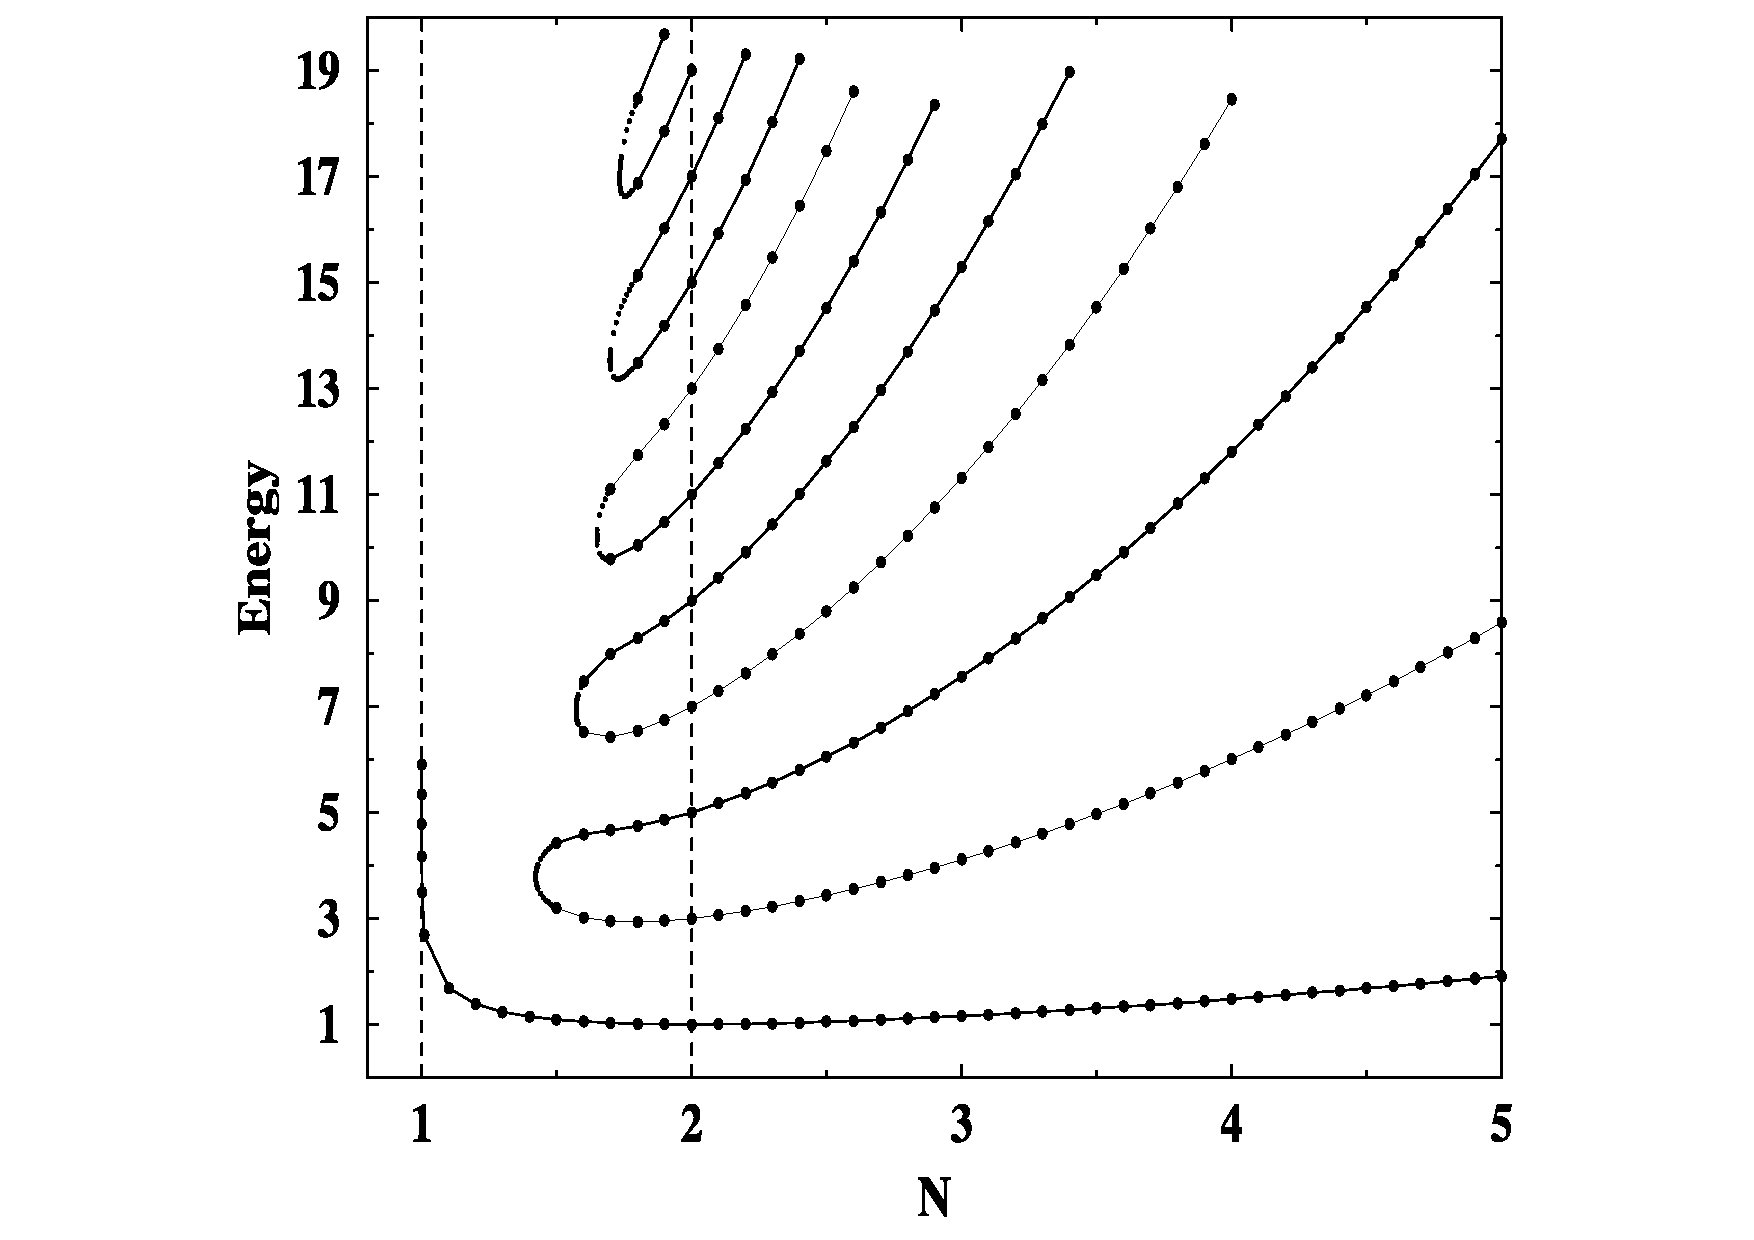
\includegraphics[width=8cm]{fig1.pdf}
\captionsetup{labelsep=none}
\caption{. Energias (autovalores) do Hamiltoniano descrito pela Eq. \eqref{hamil} em função de $N$. Para $N = 2$, obtemos o oscilador harmônico simples que possui energias $E_n = 2n + 1$. Para $N \geq 2$, os autovalores são reais, positivos e discretos, mesmo o Hamiltoniano não sendo hermitiano. Para $N\leq 2$, os autovalores são parcialmente complexos e formam pares complexos conjugados. [C. M Bender and S. Boettcher, Phys. Rev. Lett. \textbf{80} 5243 (1998)] }
\end{figure}
Curiosamente, quando $N\geq 2$ os autovalores são reais, discretos e positivos, mesmo quando o Hamiltoniano não é hermitiano! Antes da década de 90, a consideração de Hamiltonianos imaginários seria uma ideia absurda visto que eles não podem ser Hermitianos e contrariariam um dos postulados fundamentais da teoria quântica. No entanto, o postulado da hermiticidade foi colocado apenas pela sua garantia de que operadores Hermitianos possuem um espectro real de autovalores. Com a descoberta de outros operadores que, mesmo não sendo Hermitianos, possuem espectro reais, começamos a questionar a criação de um novo formalismo, mais geral, e que possa ser utilizado para descrever sistemas da natureza.

Olhando novamente para a Fig. 1, quando $N \leq 2$, no entanto, os autovalores formam pares de números complexos cujas partes imaginárias são opostas, isto é, $a \pm bi$, ditos pares complexos conjugados. Para $1 < N < 2$, existe um número finito de autovalores reais (mostrados no gráfico) e um número infinito de autovalores complexos (que não aparecem no gráfico). Quando $N < 1$, todos os autovalores são complexos. Na região $1 \leq N < 2$ dizemos que houve uma \textbf{quebra espontânea de simetria}. A borda que separa os dois casos ocorre exatamente no oscilador harmônico simples.

O exemplo discutido nessa seção serve também para ilustrar uma característica bem geral encontrada em operadores não-Hermitianos. Se o Hamiltoniano depende de um parâmetro $\beta$, os autovalores do operador são divididos em duas fases. Quando $\beta > \beta_c$, onde $\beta_c$ é um valor crítico do parâmetro $\beta$, todos os autovalores são reais. A nomenclatura não é uniforma mas podemos chamar essa situação de \textbf{fase inteira}. Por outro lado, quando $\beta < \beta_c$ os autovalores se tornam complexos (parcial ou inteiramente) e chamamos esa situação de \textbf{fase quebrada}. A evolução temporal de um estado descrito por um operador com simetria $PT$ depende de forma crucial da fase do Hamiltoniano, como iremos ver na seção 4.

\subsection{O Caso $N = 4$}

Um caso muito curioso com relação ao Hamiltoniano \eqref{hamil} ocorre quando $N = 4$. Nesse caso, o potencial onde se encontra a partícula está ``de cabeça para baixo'' (\textit{upside-down potential}):
\begin{equation}
    H = P^2 - X^4.
    \label{upside}
\end{equation}
Se uma partícula clássica estivesse sob ação de um campo de força descrito por esse potencial, nossa intuição diz que ela ocuparia uma posição instável e, consequentemente, a força empurraria a partícula para $\pm \infty$ no decorrer do tempo. Do ponto de vista da teoria quântica, essa partícula não poderia ser descrita por uma função de onda localizada, já que ela teria uma probabilidade finita de ocupar qualquer posição no eixo $x$ em qualquer tempo $t$. No entanto, o gráfico da Figura 1 mostra que a versão quântica é descrita por uma função de onda localizada com energias positivas e discretas! Para explicar esse comportamento, observe primeiramente que para um Hamiltoniano complexo, forças complexas (imaginárias) estarão atuando sob a partícula. Assim, se quisermos compreender a dinâmica do sistema é necessário estender nossa análise para o domínio complexo da posição. O movimento da partícula é descrito agora não somente no eixo $x$ real mas sim no plano complexo $\text{Re}(x) + i\text{Im}(x)$. Uma vez no plano complexo, não faz sentido dizer que um número imaginário é maior ou menor que o outro, isto é, no domínio dos números complexos não existe a noção de maior ou menor que. O número 2+3i é maior ou menor que 3-5i? Como a noção de máximo ou mínimo de um potencial na linha real é justificada pela noção de maior ou menor que, no plano complexo não podemos definir um potencial instável ou estável. De fato, uma análise mais profunda demonstra que, para o potencial \eqref{upside} a partícula passa a maior parte do seu tempo \textbf{na origem}. Isso explica o autovalor real de energia e consequentemente uma função de onda localizada para a partícula.

Pode-se olhar portanto para a teoria quântica não-Hermitiana como uma extensão da teoria quântica convencional para o domínio do plano complexo. Com isso, temos uma nova maneira de olhar para determinados problemas e inferir uma dinâmica nova e, na maioria das vezes, surpreendente. As ideias apontadas até aqui para um Hamiltoniano quântico podem ser estendidas para o domínio clássico da mecânica. O próprio Bender calculou várias trajetórias no domínio complexo da posição para Hamiltonianos clássicos com simetria $PT$.


\section{Um Aparente Paradoxo}

Vamos apresentar agora uma ``prova'' de que um operador com simetria de paridade e reversão temporal em conjunto possui autovalores reais. Para isso, considere o Hamiltoniano que comuta com o operador $PT$: $[H,PT] = 0$. Operadores que comutam compartilham a mesma base, de forma que podemos escrever
\begin{align*}
 PT\phi             &= \lambda\phi                &   H\phi  &= E \phi \\
 PTPT\phi   &= PT\lambda\phi      &   PTH\phi  &= PTE \phi \\
 P^2 T^2 \phi       &= \lambda^* PT\phi   &   HPT\phi  &= E^* PT \phi \\
 \phi                       &= \lambda^* \lambda \phi     &   H\phi  &= E^* \phi \\ 
 |\lambda|^2 &= 1                                          &   E  &= E^* \hspace{0.5cm} \text{(???)}
\end{align*}
A derivação acima mostra que os autovalores do Hamiltoniano são reais se o Hamiltoniano comuta com o operador conjunto $PT$. No entanto, o Hamiltoniano \eqref{hamil} satisfaz esse pré-requisito e como podemos observar na Figura 1, nem todos os autovalores são reais! Temos portanto um aparente paradoxo. A solução desse problema tem relação, claro, com o operador de inversão temporal $T$ que, como vimos, é antilinear. Quando um operador antilinear comuta com outro operador, a prova acima não conta toda a história. Esse ponto não é enfatizado em cursos de teoria quântica mas somos obrigados a apontar essa sutileza porque o aluno pode ser levado à achar a ``prova'' acima como verdadeira (assim como ele faz com os operadores Hermitianos). 


\section{Sistemas Abertos e Fechados}

Vamos demonstrar nesta seção que sistemas não-Hermitianos com simetria $PT$ são um meio-termo entre sistemas completamente abertos e sistemas completamente fechados. Para isso, considere inicialmente um sistema $A$ descrito pela matriz hamiltoniana
\begin{equation}
    H_A = [ic],
\end{equation}
onde $a$ é um número real positivo. Como o hamiltoniano não depende do tempo, o operador evolução temporal é facilmente calculado como sendo
\begin{equation}
    U(t) = e^{-i\frac{H_A}{\hbar}t} = e^{\frac{c}{\hbar}t} \rightarrow \infty \hspace{0.5cm} \text{quando} \hspace{0.5cm} t\rightarrow\infty
\end{equation}
de forma que a norma $\braket{\alpha(t)|\alpha(t)}$ do vetor no tempo $t$ tende a aumentar indefinidamente. Isso significa que o sistema $A$ é aberto e probabilidade flui para dentro do sistema, como mostra a Figura 2.
\begin{figure}[h]
\centering
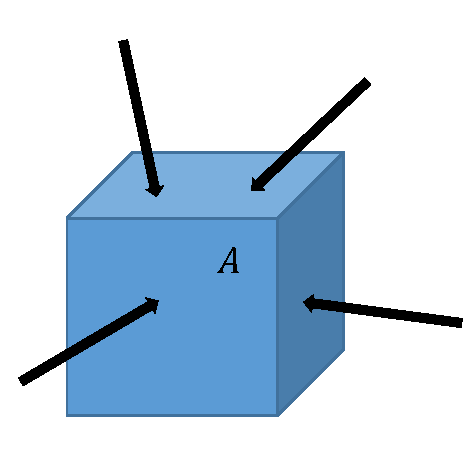
\includegraphics[width=4cm]{fig2.pdf}
\captionsetup{labelsep=none}
\caption{. A figura representa um sistema aberto $A$ onde um fluxo de probabilidade entra no sistema. A norma dos vetores do estado aumenta indefinidamente com o tempo, como discutido no texto. }
\end{figure}
Se um outro sistema $B$, inicialmente isolado do sistema $A$, isto é, que não interage com o sistema $A$, for descrito pelo Hamiltoniano
\begin{equation}
    H_B = [-ic],
\end{equation}
onde $c$ é o mesmo número real positivo de antes. A evolução temporal nesse caso é dada por
\begin{equation}
    U(t) = e^{-i\frac{H_B}{\hbar}t} = e^{-\frac{c}{\hbar}t} \rightarrow 0 \hspace{0.5cm} \text{quando} \hspace{0.5cm} t\rightarrow\infty.
\end{equation}
Nesse caso, a norma de um vetor de estado durante o tempo $t$ diminui até atingir zero para $t$ grande. Isso quer dizer que existe um fluxo de probabilidade para fora do sistema $B$, como ilustra a Figura 3.
\begin{figure}[h]
\centering
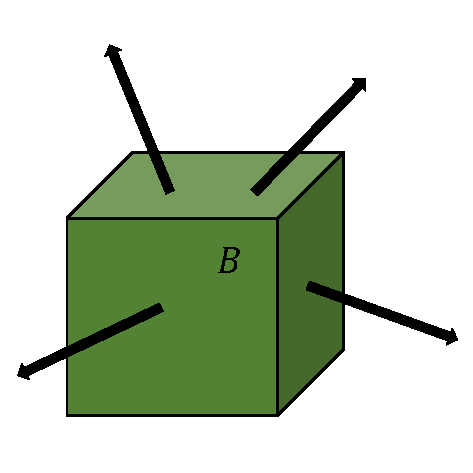
\includegraphics[width=4cm]{fig3.pdf}
\captionsetup{labelsep=none}
\caption{. A figura representa um sistema aberto $B$ onde um fluxo de probabilidade sai do sistema. A norma dos vetores do estado diminui com o tempo, como discutido no texto. }
\end{figure}
Em ambos os casos, os hamiltonianos não são Hermitianos e não esperamos uma evolução unitária (com a norma conservada). Não há nada de novo até aqui. Mas suponha que conectamos o sistema $A$ com o sistema $B$. Nesse caso, o fluxo de probabilidade (que pode ser de energia, partículas, etc) que entra no sistema $A$ será proveniente apenas do sistema $B$ (que perde energia, ou partículas, etc). Se introduzirmos a constante de acoplamento $g$ (número real), então a matriz Hamiltoniana para o sistema completo pode ser escrita como
\begin{equation}
    H_{AB} = \begin{bmatrix}
    ic & g \\
    g & -ic
\end{bmatrix}
\label{open}
\end{equation}
que \textbf{não é Hermitiana} mas sim $PT$-simétrica. É fácil verificar esse fato se lembrarmos que o operador de paridade tem a representação matricial
\begin{equation}
    P = \begin{bmatrix}
    0 & 1 \\
    1 & 0
\end{bmatrix}
\end{equation}
e o operador inversão temporal $T$ apenas troca $i$ por $-i$. Assim, fica como exercício para o aluno demonstrar que $[H_{AB},PT] = 0$. Infelizmente o cálculo da evolução temporal diretamente do hamiltoniano \eqref{open} é bastante complicado. Porém, é fácil calcular as energias do sistema:
\begin{equation}
    E_{\pm} = \pm \sqrt{g^2 - c^2}.
\end{equation}
Note que se $g > c$, as energias são positivas e que se $g<c$ as energias são complexas formando pares conjugados. Esse é um exemplo explícito e muito raro onde podemos calcular de maneira analítica as energias de um sistema não-Hermitiano com simetria $PT$. Nesse caso, o ponto de quebra de simetria é $g = c$. Podemos notar dois pontos importantes nesse simples exemplo:
\begin{enumerate}
    \item A taxa de perda/ganho de probabilidade do sistema $A$ e $B$ são iguais a $c$.
    \item Sistemas com simetria $PT$ situam-se entre sistemas abertos e fechados.
\end{enumerate}
O primeiro ponto é muito importante e tem a ver com as próprias simetrias do sistema. Suponha que o hamiltoniano do sistema $B$ fosse $-di$ no lugar de $-ic$ onde $d > 0$. Nesse caso, é fácil verificar que a matriz resultante \eqref{open} não possui mais a simetria $PT$ (verifique!). Fisicamente o que acontece é que a simetria de paridade inverte a posição dos dois sistemas. Se aplicarmos somente essa simetria, ainda conseguimos distinguir os dois sistemas pois um deles perde e o outro ganha probabilidade. Assim, quando aplicamos a simetria de inversão temporal, se os dois sistemas tivessem taxas de ganho e perda de probabilidade diferentes, ainda conseguiríamos distingui-los. Por isso ambos devem possuir a mesma taxa $c$.

Por muito tempo considerou-se a perda existente em sistemas físicos como um fator desagradável e não desejável para se ter num determinado dispositivo. Com a introdução da simetria $PT$, vemos que é possível criar uma nova dinâmica em sistemas com ganho e perda equilibrados. Iremos tocar nesse ponto na seção 7 quando aplicarmos essas ideias em sistemas ópticos, onde foi comprovado inicialmente as propriedades de sistemas $PT$-simétricos.


\section{Evolução Temporal de um Sistema $PT$-simétrico}

Após identificar a simetria responsável pela realidade dos autovalores de um operador $PT$-simétrico, Bender estudou a evolução temporal regida por tal Hamiltoniano. Vale lembrar que um dos postulados da mecânica quântica exige uma evolução unitária de modo a se obter uma probabilidade conservada num sistema fechado. Como na região com a fase quebrada os autovalores são complexos, não tem como gerar, nessa situação, uma evolução unitária e portanto devemos construir uma teoria quântica apenas para a fase inteira do Hamiltoniano. Acontece que essa pergunta só foi respondida bem depois da publicação do trabalho original de 1998. A grande dificuldade encontrada por Bender foi a falta de uma outra simetria que sempre está presente quando o hamiltoniano está na sua fase inteira, isto é, com os autovalores reais. Essa nova simetria, representada pelo operador $C$, não será discutida aqui pois requer um conhecimento mais aprofundado das técnicas matemáticas que vai além do nível desta aula. Mas é possível demonstrar que é possível montar uma teoria quântica, na fase inteira de um Hamiltoniano, tal que sua evolução temporal respeite as regras da mecânica quântica. Em outras palavras, é sempre possível montar um operador de evolução temporal unitário para um Hamiltoniano $PT$-simétrico desde que ele se encontre na fase inteira com autovalores reais. O aluno que quiser se aprofundar mais nesse quesito, pode consultar as referências listadas no plano de aula. 




\section{Aplicações em Sistemas Fotônicos}

Curiosamente, a primeira verificação experimental das propriedades de um sistema com simetria de paridade e inversão temporal veio de fora do campo da quântica. A fotônica foi a área de pesquisa responsável pela primeira implementação em laboratório de um sistema material com simetria $PT$ interagindo com o campo eletromagnético. Como isso foi possível? Todos os aspectos do eletromagnetismo clássico são descritos pelas equações de Maxwell, como o estudante deve estar ciente. É possível, no entanto, através de várias aproximações, demonstrar que a propagação do campo elétrico $E(x,z)$ através de um material com índice de refração não-homogêneo e complexo $n(x) = n_0 + n_R(x) + in_I(x)$ é governada pela equação paraxial da onda
\begin{equation}
    i\frac{\partial E}{\partial z} =\frac{1}{2k}\frac{\partial^2 E }{\partial x^2} + V(x)E,
\end{equation}
onde $k = k_0 n_0$, $k_0 = 2\pi/\lambda$ com $\lambda$ sendo o comprimento de onda no vácuo. O ``potencial'' aparecendo na equação paraxial é na verdade proporcional ao índice de refração do material:
\begin{equation}
    V(x) = k_0 [n_R(x) + in_I(x)].
\end{equation}
Para que o material possua simetria $PT$ vimos que o Hamiltoniano deve ser invariante $x\rightarrow -x$ e $i\rightarrow -i$, ou seja, devemos ter $V^* (-x) = V(x)$. Em termos do índice de refração:
\begin{align}
        V^* (-x) &= V(x) \\
        k_0 [n_R(-x) - in_I(-x)] &= k_0 [n_R(x) + in_I(x)],\\
\end{align}
\begin{empheq}[box=\tcbhighmath]{equation}
n_R (-x) = n_R(x) \hspace{0.5cm} \text{e} \hspace{0.5cm} n_I(-x) = -n_I(x)
\end{empheq}
Ou seja, a parte real do índice de refração deve ser par e a parte imaginária deve ser ímpar para que o sistema fotônico possua simetria $PT$. Como a parte imaginária do índice de refração está relacionada ao ganho e à perda de energia da onda eletromagnética, é necessário introduzir materiais que forneçam energia ao campo e, ao mesmo tempo, retirem energia do mesmo. No entanto, criar num laboratório materiais que apresentem ganho é, em geral, bem complicado. Um sistema não-Hermitiano \textbf{possuindo apenas perdas ópticas} foi realizado experimentalmente por A. Guo e colaboradores em 2009. Os pesquisadores criaram uma estrutura formada por dois guias de onda, onde ambos os guias possuiam perda. A diferença é que um dos guias continha uma perda modulada. Isto é, a luz era absorvida de forma diferente em diferentes posições do guia. O sistema não possui ganho. A grandeza medida no laboratório foi a transmissão da energia da onda que se propagou através dos guias e sobreviveu na saída. Num sistema hermitiano, espera-se que quanto maior a perda no sistema, menor a transmissão de energia. Os autores mostraram, entretanto, que a transmissão poderia aumentar com o aumento da perda no sistema óptico. Isso é bastante contraintuitivo e é apenas um exemplo da grande importância que sistemas não-Hermitianos podem desempenhar na aplicação de dispositivos fotônicos, por exemplo.


\begin{figure}[h]
\centering
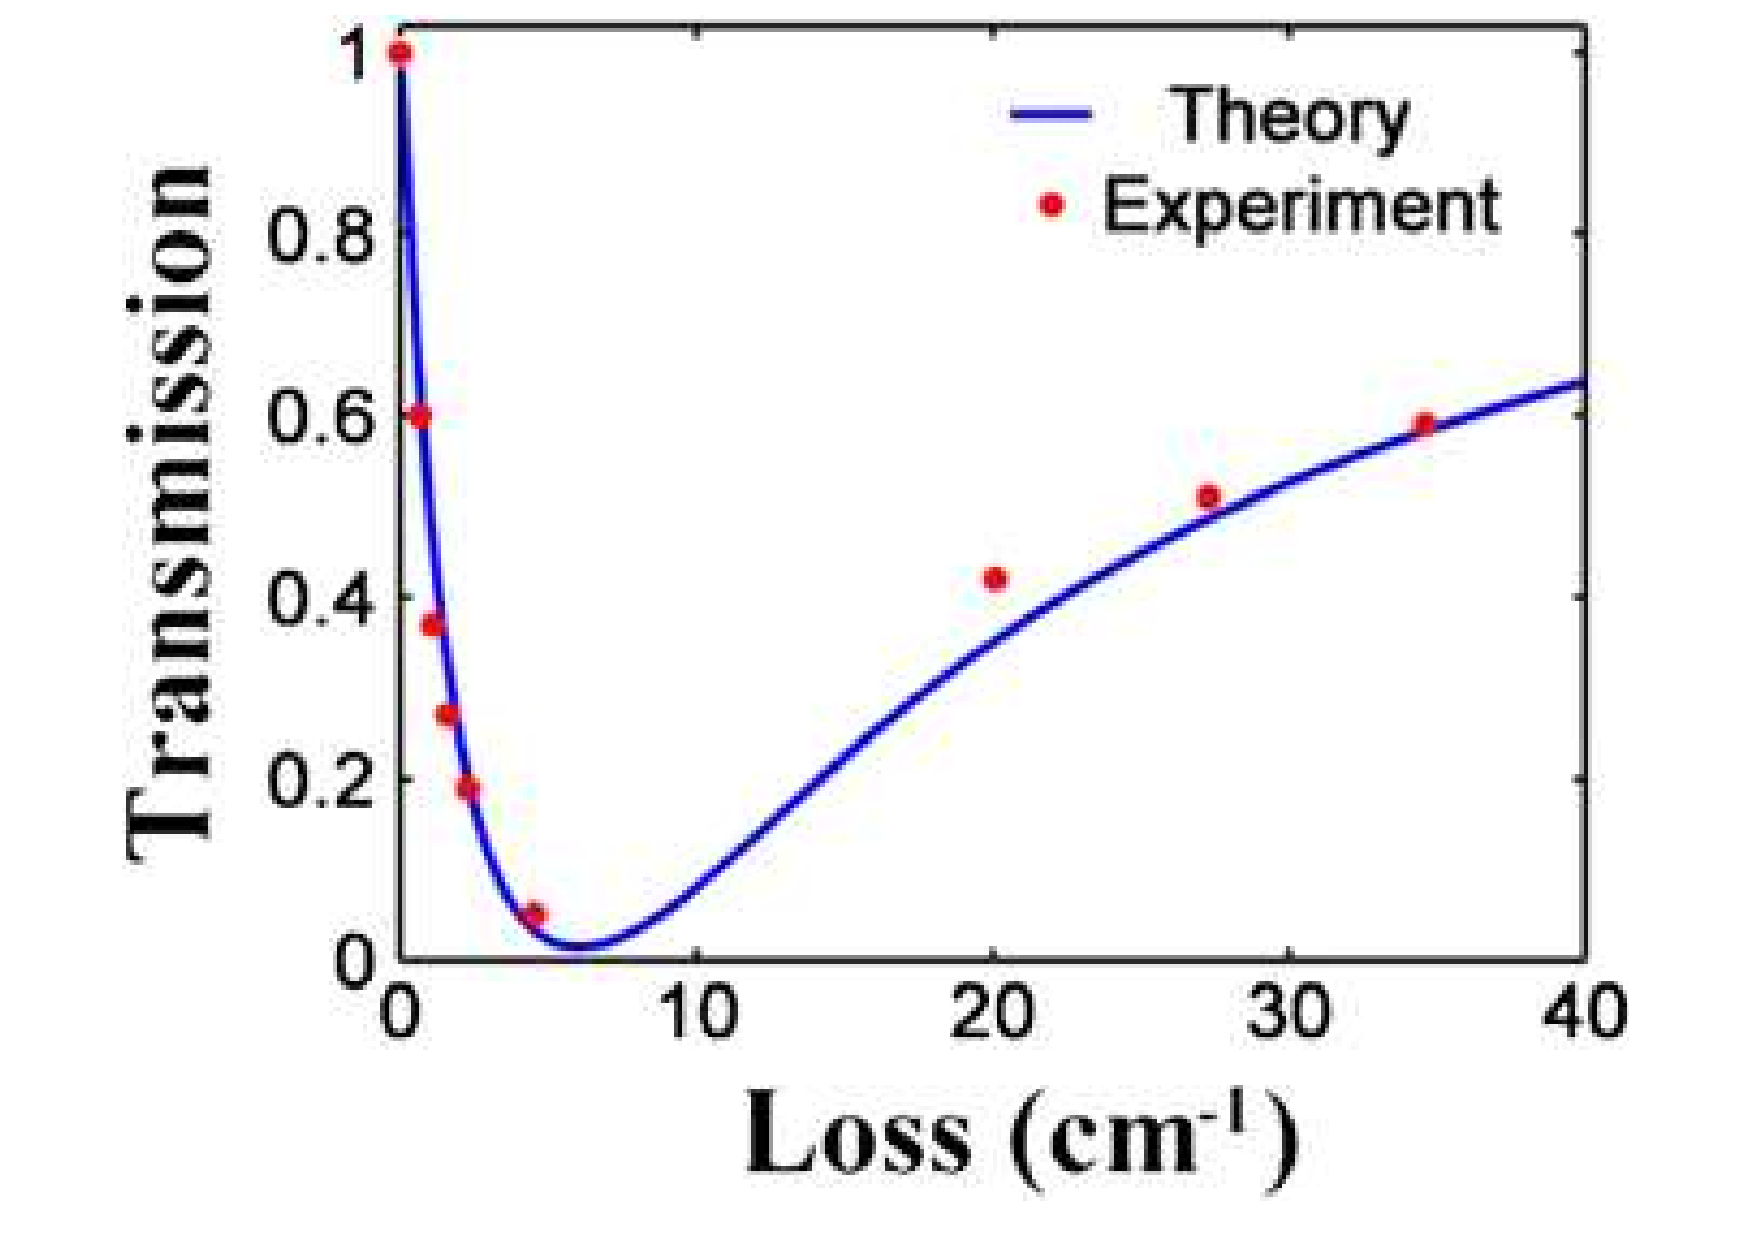
\includegraphics[width=7cm]{fig4.pdf}
\captionsetup{labelsep=none}
\caption{. Observação experimental da transmissão de luz através de um par acoplado de guidas de onda com simetria $PT$ em função da perda presente em um dos guias. A linha azul é o resultado obtido através das equações de Maxwell e os pontos em vermelho são os resultados experimentais. [A. Guo et. al., Phys. Rev. Lett. \textbf{103} 093902 (2009)] }
\end{figure}



\section{Conclusões}

O estudo dos sistemas não-Hermitianos ainda está no início e é esperado inúmeras descobertas em várias áreas de pesquisa nos próximos anos. Por muito tempo considerou-se a utilização de operadores Hermitianos como a única opção viável para descrever sistemas físicos. Nessa aula, mostrei de uma forma bem simples que essa premissa escrita em cada livro de mecânica quântica pode ser relaxada em certas situações. De uma visão mais geral, operadores não-Hermitianos são generalizações das teorias hermitianas para o espaço complexo. Com isso, novas abordagens e interpretações aparecem para enriquecer ainda mais a física já conhecida. O papel da simetria $PT$ nos sistemas físicos certamente veio para ficar e apenas o futuro dirá as possíveis reviravoltas proporcionadas por essa teoria.





















































\end{document}
